\PassOptionsToPackage{unicode=true}{hyperref} % options for packages loaded elsewhere
\PassOptionsToPackage{hyphens}{url}
%
\documentclass[]{article}
\usepackage{lmodern}
\usepackage{amssymb,amsmath}
\usepackage{ifxetex,ifluatex}
\usepackage{fixltx2e} % provides \textsubscript
\ifnum 0\ifxetex 1\fi\ifluatex 1\fi=0 % if pdftex
  \usepackage[T1]{fontenc}
  \usepackage[utf8]{inputenc}
  \usepackage{textcomp} % provides euro and other symbols
\else % if luatex or xelatex
  \usepackage{unicode-math}
  \defaultfontfeatures{Ligatures=TeX,Scale=MatchLowercase}
\fi
% use upquote if available, for straight quotes in verbatim environments
\IfFileExists{upquote.sty}{\usepackage{upquote}}{}
% use microtype if available
\IfFileExists{microtype.sty}{%
\usepackage[]{microtype}
\UseMicrotypeSet[protrusion]{basicmath} % disable protrusion for tt fonts
}{}
\IfFileExists{parskip.sty}{%
\usepackage{parskip}
}{% else
\setlength{\parindent}{0pt}
\setlength{\parskip}{6pt plus 2pt minus 1pt}
}
\usepackage{hyperref}
\hypersetup{
            pdftitle={GDF15 ELISA Assay for Ketogenic Diet},
            pdfauthor={Claire Gleason, Molly Carter and Dave Bridges},
            pdfborder={0 0 0},
            breaklinks=true}
\urlstyle{same}  % don't use monospace font for urls
\usepackage[margin=1in]{geometry}
\usepackage{color}
\usepackage{fancyvrb}
\newcommand{\VerbBar}{|}
\newcommand{\VERB}{\Verb[commandchars=\\\{\}]}
\DefineVerbatimEnvironment{Highlighting}{Verbatim}{commandchars=\\\{\}}
% Add ',fontsize=\small' for more characters per line
\usepackage{framed}
\definecolor{shadecolor}{RGB}{248,248,248}
\newenvironment{Shaded}{\begin{snugshade}}{\end{snugshade}}
\newcommand{\AlertTok}[1]{\textcolor[rgb]{0.94,0.16,0.16}{#1}}
\newcommand{\AnnotationTok}[1]{\textcolor[rgb]{0.56,0.35,0.01}{\textbf{\textit{#1}}}}
\newcommand{\AttributeTok}[1]{\textcolor[rgb]{0.77,0.63,0.00}{#1}}
\newcommand{\BaseNTok}[1]{\textcolor[rgb]{0.00,0.00,0.81}{#1}}
\newcommand{\BuiltInTok}[1]{#1}
\newcommand{\CharTok}[1]{\textcolor[rgb]{0.31,0.60,0.02}{#1}}
\newcommand{\CommentTok}[1]{\textcolor[rgb]{0.56,0.35,0.01}{\textit{#1}}}
\newcommand{\CommentVarTok}[1]{\textcolor[rgb]{0.56,0.35,0.01}{\textbf{\textit{#1}}}}
\newcommand{\ConstantTok}[1]{\textcolor[rgb]{0.00,0.00,0.00}{#1}}
\newcommand{\ControlFlowTok}[1]{\textcolor[rgb]{0.13,0.29,0.53}{\textbf{#1}}}
\newcommand{\DataTypeTok}[1]{\textcolor[rgb]{0.13,0.29,0.53}{#1}}
\newcommand{\DecValTok}[1]{\textcolor[rgb]{0.00,0.00,0.81}{#1}}
\newcommand{\DocumentationTok}[1]{\textcolor[rgb]{0.56,0.35,0.01}{\textbf{\textit{#1}}}}
\newcommand{\ErrorTok}[1]{\textcolor[rgb]{0.64,0.00,0.00}{\textbf{#1}}}
\newcommand{\ExtensionTok}[1]{#1}
\newcommand{\FloatTok}[1]{\textcolor[rgb]{0.00,0.00,0.81}{#1}}
\newcommand{\FunctionTok}[1]{\textcolor[rgb]{0.00,0.00,0.00}{#1}}
\newcommand{\ImportTok}[1]{#1}
\newcommand{\InformationTok}[1]{\textcolor[rgb]{0.56,0.35,0.01}{\textbf{\textit{#1}}}}
\newcommand{\KeywordTok}[1]{\textcolor[rgb]{0.13,0.29,0.53}{\textbf{#1}}}
\newcommand{\NormalTok}[1]{#1}
\newcommand{\OperatorTok}[1]{\textcolor[rgb]{0.81,0.36,0.00}{\textbf{#1}}}
\newcommand{\OtherTok}[1]{\textcolor[rgb]{0.56,0.35,0.01}{#1}}
\newcommand{\PreprocessorTok}[1]{\textcolor[rgb]{0.56,0.35,0.01}{\textit{#1}}}
\newcommand{\RegionMarkerTok}[1]{#1}
\newcommand{\SpecialCharTok}[1]{\textcolor[rgb]{0.00,0.00,0.00}{#1}}
\newcommand{\SpecialStringTok}[1]{\textcolor[rgb]{0.31,0.60,0.02}{#1}}
\newcommand{\StringTok}[1]{\textcolor[rgb]{0.31,0.60,0.02}{#1}}
\newcommand{\VariableTok}[1]{\textcolor[rgb]{0.00,0.00,0.00}{#1}}
\newcommand{\VerbatimStringTok}[1]{\textcolor[rgb]{0.31,0.60,0.02}{#1}}
\newcommand{\WarningTok}[1]{\textcolor[rgb]{0.56,0.35,0.01}{\textbf{\textit{#1}}}}
\usepackage{longtable,booktabs}
% Fix footnotes in tables (requires footnote package)
\IfFileExists{footnote.sty}{\usepackage{footnote}\makesavenoteenv{longtable}}{}
\usepackage{graphicx,grffile}
\makeatletter
\def\maxwidth{\ifdim\Gin@nat@width>\linewidth\linewidth\else\Gin@nat@width\fi}
\def\maxheight{\ifdim\Gin@nat@height>\textheight\textheight\else\Gin@nat@height\fi}
\makeatother
% Scale images if necessary, so that they will not overflow the page
% margins by default, and it is still possible to overwrite the defaults
% using explicit options in \includegraphics[width, height, ...]{}
\setkeys{Gin}{width=\maxwidth,height=\maxheight,keepaspectratio}
\setlength{\emergencystretch}{3em}  % prevent overfull lines
\providecommand{\tightlist}{%
  \setlength{\itemsep}{0pt}\setlength{\parskip}{0pt}}
\setcounter{secnumdepth}{5}
% Redefines (sub)paragraphs to behave more like sections
\ifx\paragraph\undefined\else
\let\oldparagraph\paragraph
\renewcommand{\paragraph}[1]{\oldparagraph{#1}\mbox{}}
\fi
\ifx\subparagraph\undefined\else
\let\oldsubparagraph\subparagraph
\renewcommand{\subparagraph}[1]{\oldsubparagraph{#1}\mbox{}}
\fi

% set default figure placement to htbp
\makeatletter
\def\fps@figure{htbp}
\makeatother


\title{GDF15 ELISA Assay for Ketogenic Diet}
\author{Claire Gleason, Molly Carter and Dave Bridges}
\date{January 2, 2018}

\begin{document}
\maketitle

{
\setcounter{tocdepth}{2}
\tableofcontents
}
\hypertarget{purpose}{%
\section{Purpose}\label{purpose}}

To determine the levels of GDF15 from either ketogenic diet or
dexamethasone treatments.

\hypertarget{experimental-details}{%
\section{Experimental Details}\label{experimental-details}}

Used the Quantikine kit, used 15 uL serum rather than 50 uL.

\hypertarget{raw-data}{%
\section{Raw Data}\label{raw-data}}

The input data is calculated from MyAssays from a four parameter
logistic regression calculation (\url{https://www.myassays.com/}) and
annotated with cohort, sex and groups. The equation (solved for
concentration) is:

\[ Concentration = c\left ( \frac{a-d}{y-d} -1 \right )^{\frac{1}{b}} \]

These data can be found in
\textbf{/Users/davebrid/Documents/GitHub/TissueSpecificTscKnockouts/Mouse
Data/Ketogenic Diets} in a file named \textbf{GDF15 ELISA Results.csv}.
This script was most recently updated on \textbf{Mon Apr 6 11:01:47
2020}.

\hypertarget{analysis}{%
\section{Analysis}\label{analysis}}

\hypertarget{ketogenic-diets}{%
\subsection{Ketogenic Diets}\label{ketogenic-diets}}

We had serum from the two cohorts of ketogenic mice, some with males and
females

\begin{verbatim}
## 
##  Shapiro-Wilk normality test
## 
## data:  log(subset(kd.data, Sex == "F" & Diet == "CD")$Concentration)
## W = 0.9, p-value = 0.1
\end{verbatim}

\begin{verbatim}
## 
##  Wilcoxon rank sum test with continuity correction
## 
## data:  Concentration by Diet
## W = 8, p-value = 0.07
## alternative hypothesis: true location shift is not equal to 0
\end{verbatim}

\begin{verbatim}
## 
##  Shapiro-Wilk normality test
## 
## data:  subset(kd.data, Sex == "F" & Diet == "CD")$Concentration
## W = 0.9, p-value = 0.2
\end{verbatim}

\begin{verbatim}
## 
##  Shapiro-Wilk normality test
## 
## data:  subset(kd.data, Sex == "F" & Diet == "KD")$Concentration
## W = 0.9, p-value = 0.3
\end{verbatim}

\begin{verbatim}
## Levene's Test for Homogeneity of Variance (center = median)
##       Df F value Pr(>F)
## group  1    0.05   0.82
##       11
\end{verbatim}

\begin{verbatim}
## 
##  Two Sample t-test
## 
## data:  Concentration by Diet
## t = -2, df = 11, p-value = 0.06
## alternative hypothesis: true difference in means is not equal to 0
## 95 percent confidence interval:
##  -34.12   1.06
## sample estimates:
## mean in group CD mean in group KD 
##             14.6             31.1
\end{verbatim}

\begin{verbatim}
## 
##  Shapiro-Wilk normality test
## 
## data:  subset(kd.data, Sex == "M" & Diet == "CD")$Concentration
## W = 0.9, p-value = 0.5
\end{verbatim}

\begin{verbatim}
## 
##  Shapiro-Wilk normality test
## 
## data:  subset(kd.data, Sex == "M" & Diet == "KD")$Concentration
## W = 0.9, p-value = 0.1
\end{verbatim}

\begin{verbatim}
## Levene's Test for Homogeneity of Variance (center = median)
##       Df F value Pr(>F)
## group  1    1.87   0.19
##       18
\end{verbatim}

\begin{verbatim}
## 
##  Two Sample t-test
## 
## data:  Concentration by Diet
## t = -1, df = 18, p-value = 0.2
## alternative hypothesis: true difference in means is not equal to 0
## 95 percent confidence interval:
##  -49.6  11.4
## sample estimates:
## mean in group CD mean in group KD 
##             31.2             50.3
\end{verbatim}

\begin{longtable}[]{@{}llrrr@{}}
\caption{Summary statistics for effects of a ketogenic
diet}\tabularnewline
\toprule
Diet & Sex & GDF15 & Error & N\tabularnewline
\midrule
\endfirsthead
\toprule
Diet & Sex & GDF15 & Error & N\tabularnewline
\midrule
\endhead
CD & M & 9.35 & 2.00 & 7\tabularnewline
CD & F & 4.37 & 1.78 & 7\tabularnewline
KD & M & 14.70 & 3.10 & 13\tabularnewline
KD & F & 9.01 & 1.72 & 6\tabularnewline
\bottomrule
\end{longtable}

\begin{longtable}[]{@{}lrrrr@{}}
\caption{ANOVA for effects of sex and ketogenic diet on GDF15
levels}\tabularnewline
\toprule
term & estimate & std.error & statistic & p.value\tabularnewline
\midrule
\endfirsthead
\toprule
term & estimate & std.error & statistic & p.value\tabularnewline
\midrule
\endhead
(Intercept) & 31.9 & 8.24 & 3.87 & 0.001\tabularnewline
SexF & -18.0 & 9.25 & -1.95 & 0.061\tabularnewline
DietKD & 18.0 & 9.15 & 1.97 & 0.058\tabularnewline
\bottomrule
\end{longtable}

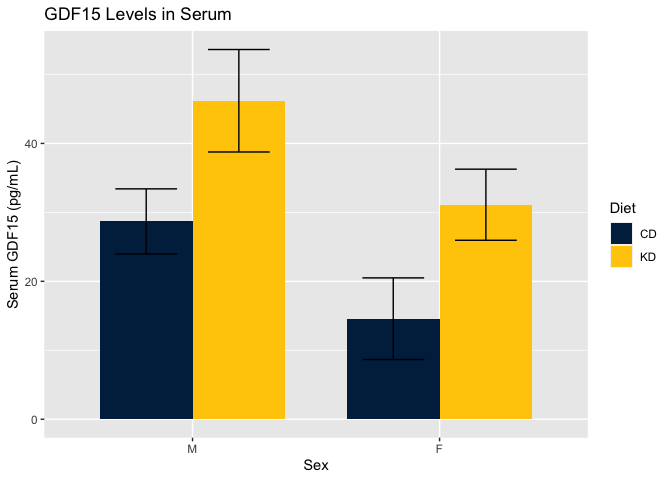
\includegraphics{figures/kd-gdf15-barplots-1.png}
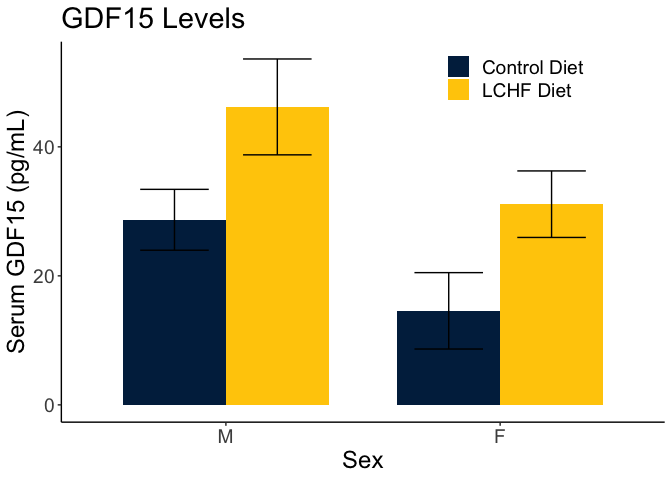
\includegraphics{figures/kd-gdf15-barplots-2.png}
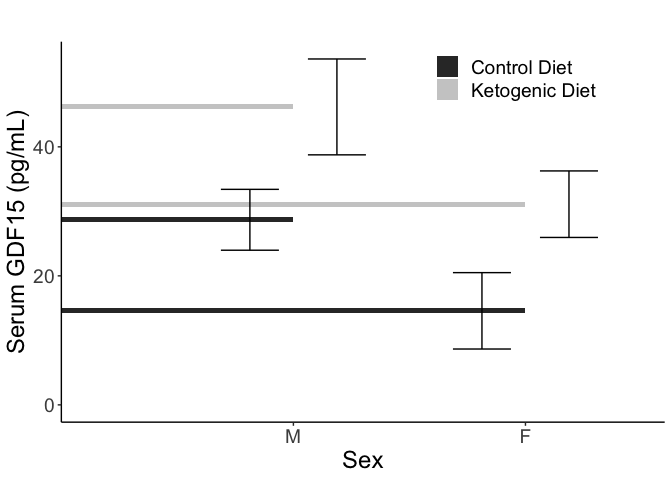
\includegraphics{figures/kd-gdf15-barplots-3.png}

We also separated the samples by cohort

\begin{figure}
\centering
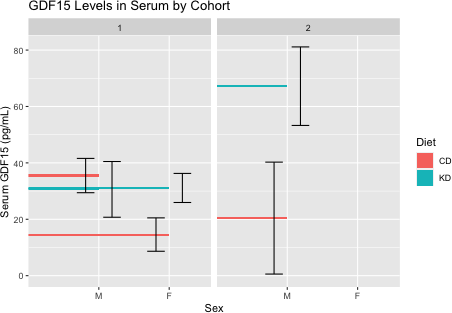
\includegraphics{figures/kd-gdf15-barplots-cohort-1.png}
\caption{Effects of Ketogenic Diet on GDF15 Levels in Serum, Separated
by Cohort}
\end{figure}

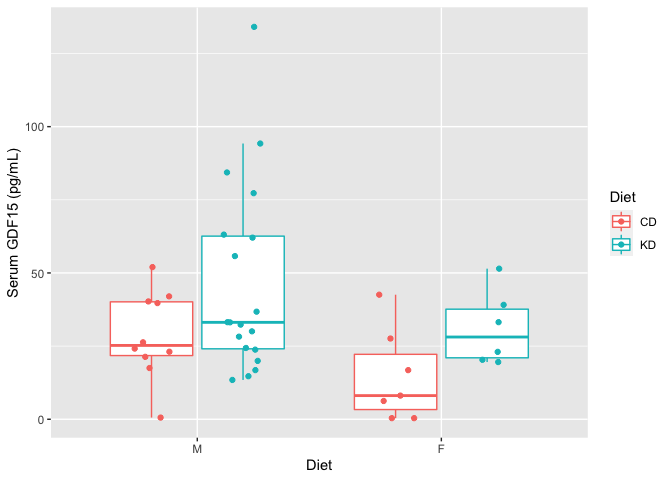
\includegraphics{figures/kd-gdf15-boxplots-1.png}
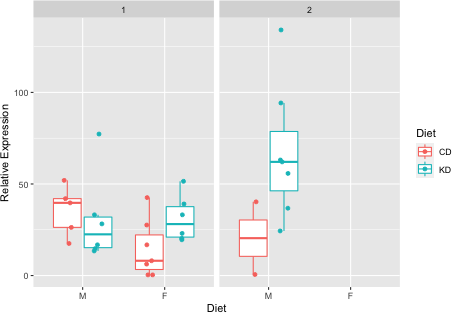
\includegraphics{figures/kd-gdf15-boxplots-2.png}

\hypertarget{interpretation}{%
\section{Interpretation}\label{interpretation}}

There was a modest increase in serum GDF15 levels in the ketogenic diets
for both sexes, inline with the liver RNAseq data. There is no clear
effect of fasting on the GDF15 levels across both sexes, diets, and
cohorts.

\hypertarget{session-information}{%
\section{Session Information}\label{session-information}}

\begin{Shaded}
\begin{Highlighting}[]
\KeywordTok{sessionInfo}\NormalTok{()}
\end{Highlighting}
\end{Shaded}

\begin{verbatim}
## R version 3.6.3 (2020-02-29)
## Platform: x86_64-apple-darwin15.6.0 (64-bit)
## Running under: macOS Catalina 10.15.3
## 
## Matrix products: default
## BLAS:   /Library/Frameworks/R.framework/Versions/3.6/Resources/lib/libRblas.0.dylib
## LAPACK: /Library/Frameworks/R.framework/Versions/3.6/Resources/lib/libRlapack.dylib
## 
## locale:
## [1] en_US.UTF-8/en_US.UTF-8/en_US.UTF-8/C/en_US.UTF-8/en_US.UTF-8
## 
## attached base packages:
## [1] stats     graphics  grDevices utils     datasets  methods   base     
## 
## other attached packages:
## [1] ggplot2_3.3.0.9000 broom_0.5.5        car_3.0-7          carData_3.0-3     
## [5] forcats_0.5.0      readr_1.3.1        dplyr_0.8.5        tidyr_1.0.2       
## [9] knitr_1.28        
## 
## loaded via a namespace (and not attached):
##  [1] zip_2.0.4         Rcpp_1.0.4        pillar_1.4.3      compiler_3.6.3   
##  [5] cellranger_1.1.0  highr_0.8         tools_3.6.3       digest_0.6.25    
##  [9] gtable_0.3.0      lattice_0.20-38   nlme_3.1-144      evaluate_0.14    
## [13] lifecycle_0.2.0   tibble_2.1.3      pkgconfig_2.0.3   rlang_0.4.5      
## [17] openxlsx_4.1.4    magick_2.3        curl_4.3          yaml_2.2.1       
## [21] haven_2.2.0       xfun_0.12         rio_0.5.16        withr_2.1.2      
## [25] stringr_1.4.0     generics_0.0.2    vctrs_0.2.4       hms_0.5.3        
## [29] grid_3.6.3        tidyselect_1.0.0  glue_1.3.2        data.table_1.12.8
## [33] R6_2.4.1          readxl_1.3.1      foreign_0.8-75    rmarkdown_2.1    
## [37] farver_2.0.3      purrr_0.3.3       magrittr_1.5      scales_1.1.0     
## [41] backports_1.1.5   htmltools_0.4.0   assertthat_0.2.1  abind_1.4-5      
## [45] colorspace_1.4-1  labeling_0.3      stringi_1.4.6     munsell_0.5.0    
## [49] crayon_1.3.4
\end{verbatim}

\end{document}
